\section{Multivariate Insights Unlocked!}

% jisne complete nahi kiya vo bhen ka loda
\section{Higher-Order Regression}

\subsection{1}
\begin{claim}
    In a simple linear regression model the point \((\overline{x},\overline{y})\) lies exactly on the least squares regression line.
\end{claim}
\begin{proof}
In a simple linear regression model, the least squares regression line is given by the equation:
\begin{align*}
    y &= Bx + A
\end{align*}
where \(B\) and \(A\) are calculated as:
\begin{align}
    B&=\frac{\sum(x_i-\overline{x})(y_i-\overline{y})}{\sum(x_i - \overline{x})^2}\\
    A&= \overline{y} - B\overline{x}\\
    \therefore y &= Bx + ( \overline{y} - B\overline{x} )
\end{align}

It is now trivial to see that point \((\overline{x},\overline{y})\) lies perfectly on the least square regression line.
\end{proof}

\subsection{2}
\begin{claim}
    The least square estimates of \(\beta_0^* = \overline{y}\) and \(\beta_1^* = \beta_1\)
\end{claim}
\begin{proof}
    In a simple linear regression model:
    \begin{align*}
        Y &= \beta_0 + \beta_1x + \epsilon\\
        \beta_1 &= \frac{\sum(x_i - \overline{x})(y_i-\overline{y})}{\sum(x_i - \overline{x})^2}\\
        \beta_0 &= \overline{y} - \beta_1\overline{x}
    \end{align*}
    while in the new model using \(z_i = x_i - \overline{x}\)
    \begin{align*}
        Y &= \beta_0^* + \beta_1^*z + \epsilon
    \end{align*}
    Using the formulae for a simple linear regression model the least square estimates of \(\beta_0^*\) and \(\beta_1^*\) are:
    \begin{align*}
        \beta_1^* &= \frac{\sum(z_i-\overline{z})(y_i-\overline{y})}{\sum(z_i - \overline{z})^2}\\
        \beta_1^* &= \frac{\sum(z_i)(y_i-\overline{y})}{\sum(z_i)^2}\\
        \beta_1^* &= \frac{\sum(x_i - \overline{x})(y_i-\overline{y})}{\sum(x_i - \overline{x})^2}\\
        \beta_1^* &= \beta_1\\
        \beta_0^* &= \overline{y} - \beta_1^*\overline{z}\\
        \beta_0^* &= \overline{y} - \beta_1^*(0)\\
        \beta_0^* &= \overline{y}
    \end{align*}
    In summary, the models are mathematically equivalent in terms of fitting the data, but the interpretation of the intercept changes. The transformed model centers the data, making the intercept equal to the mean of Y, while the slope remains the same in both models
\end{proof}

\subsection{3}
The data was run through OLS with validation split 90:10\\
\vspace{-2em}
\begin{figure}[H]
    \centering
    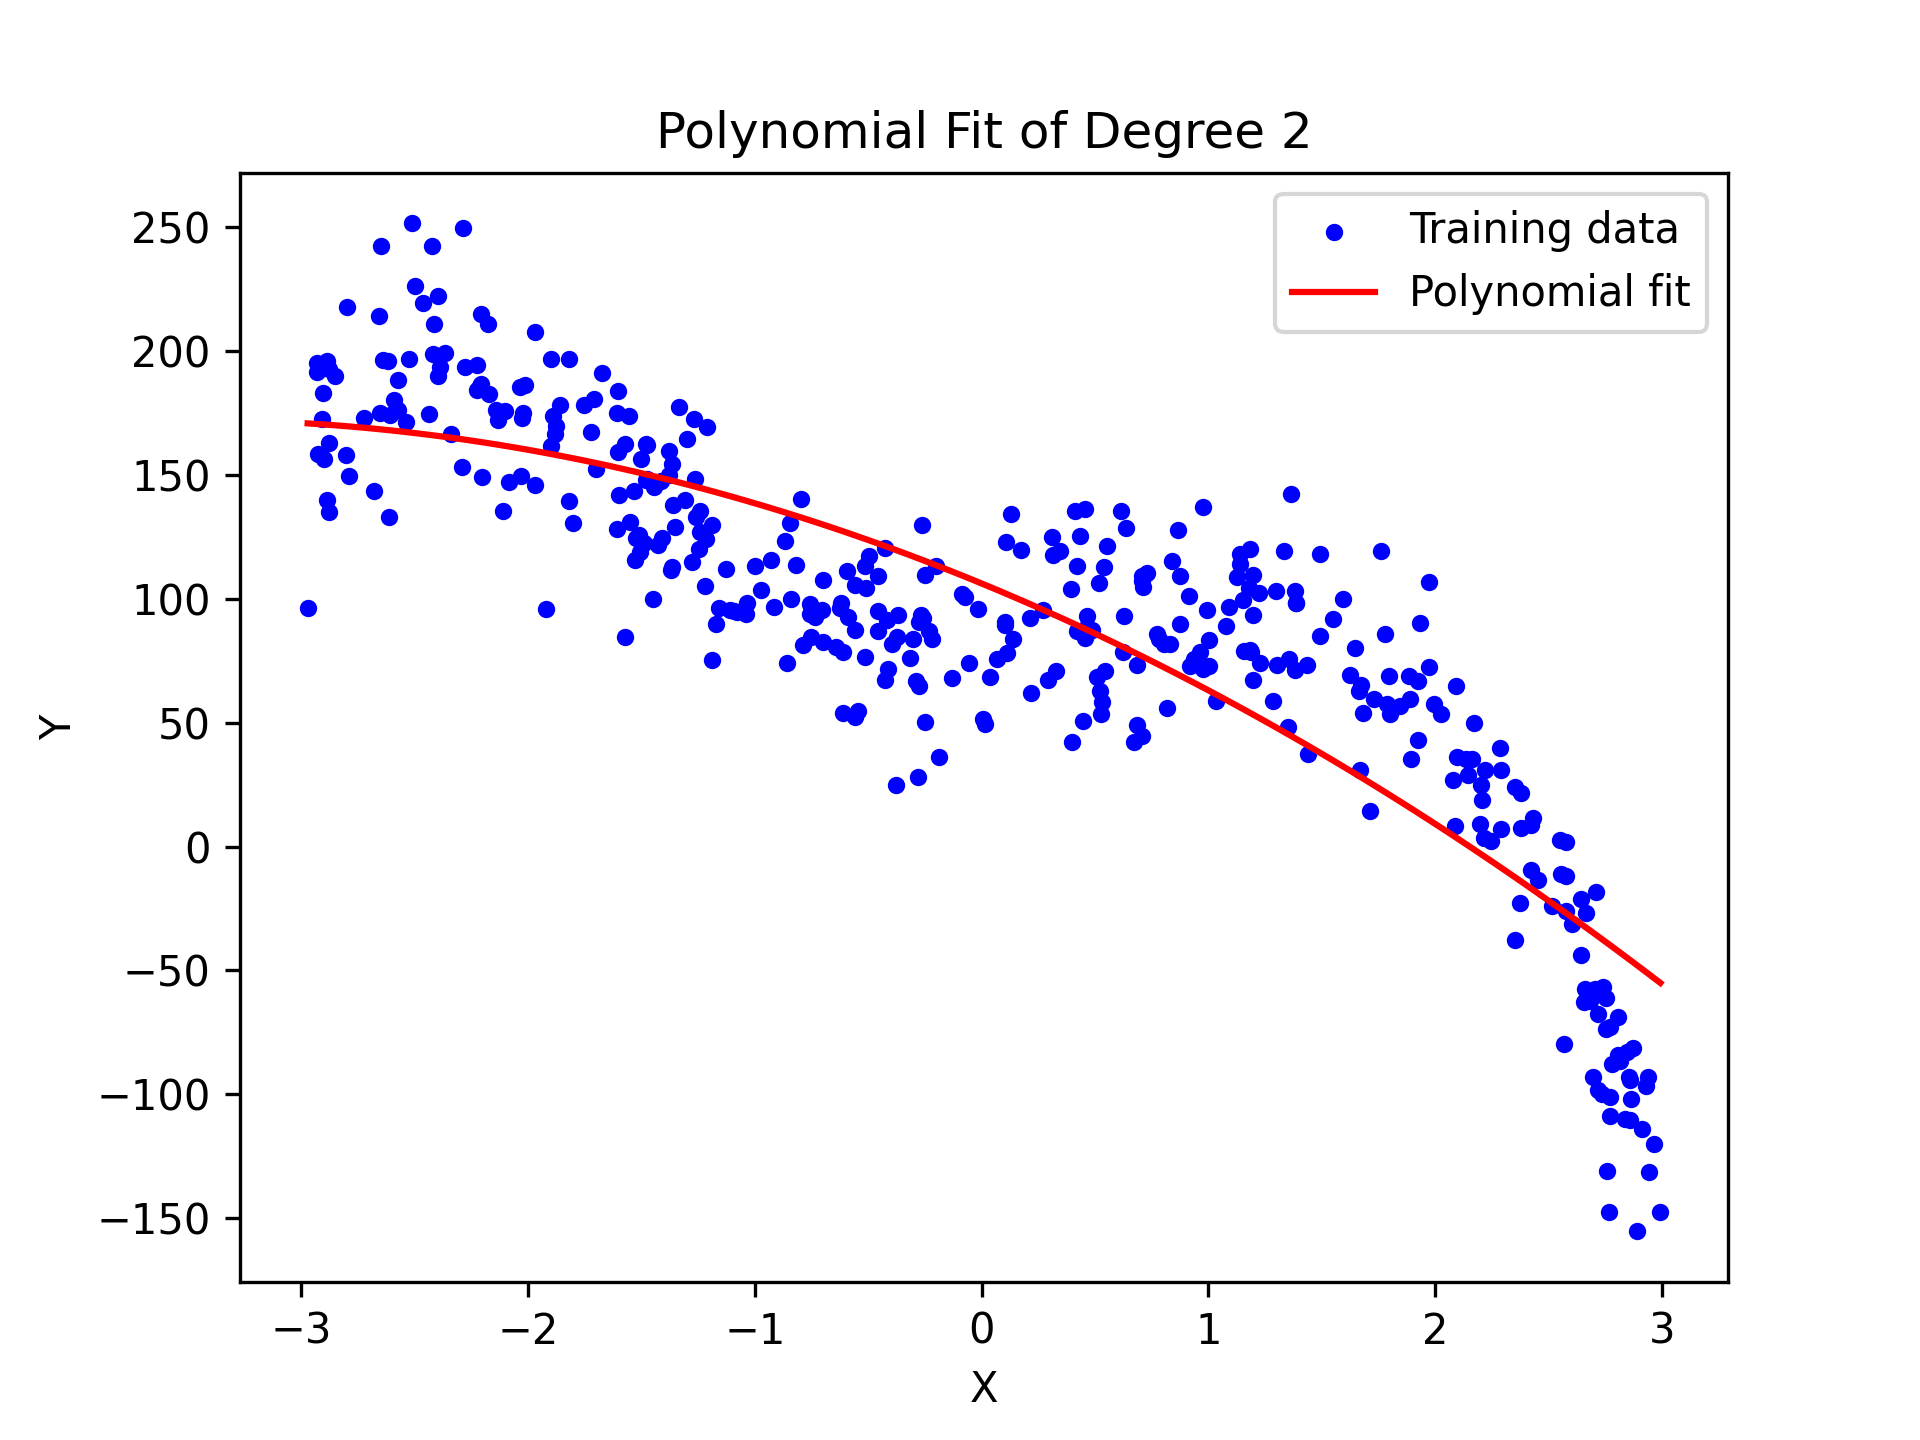
\includegraphics[width=0.5\textwidth]{./images/3/3_underfit.png}
    \vspace{-10pt}
    \caption{Underfit}
\end{figure}
\vspace{-15pt}
\begin{figure}[H]
    \centering
    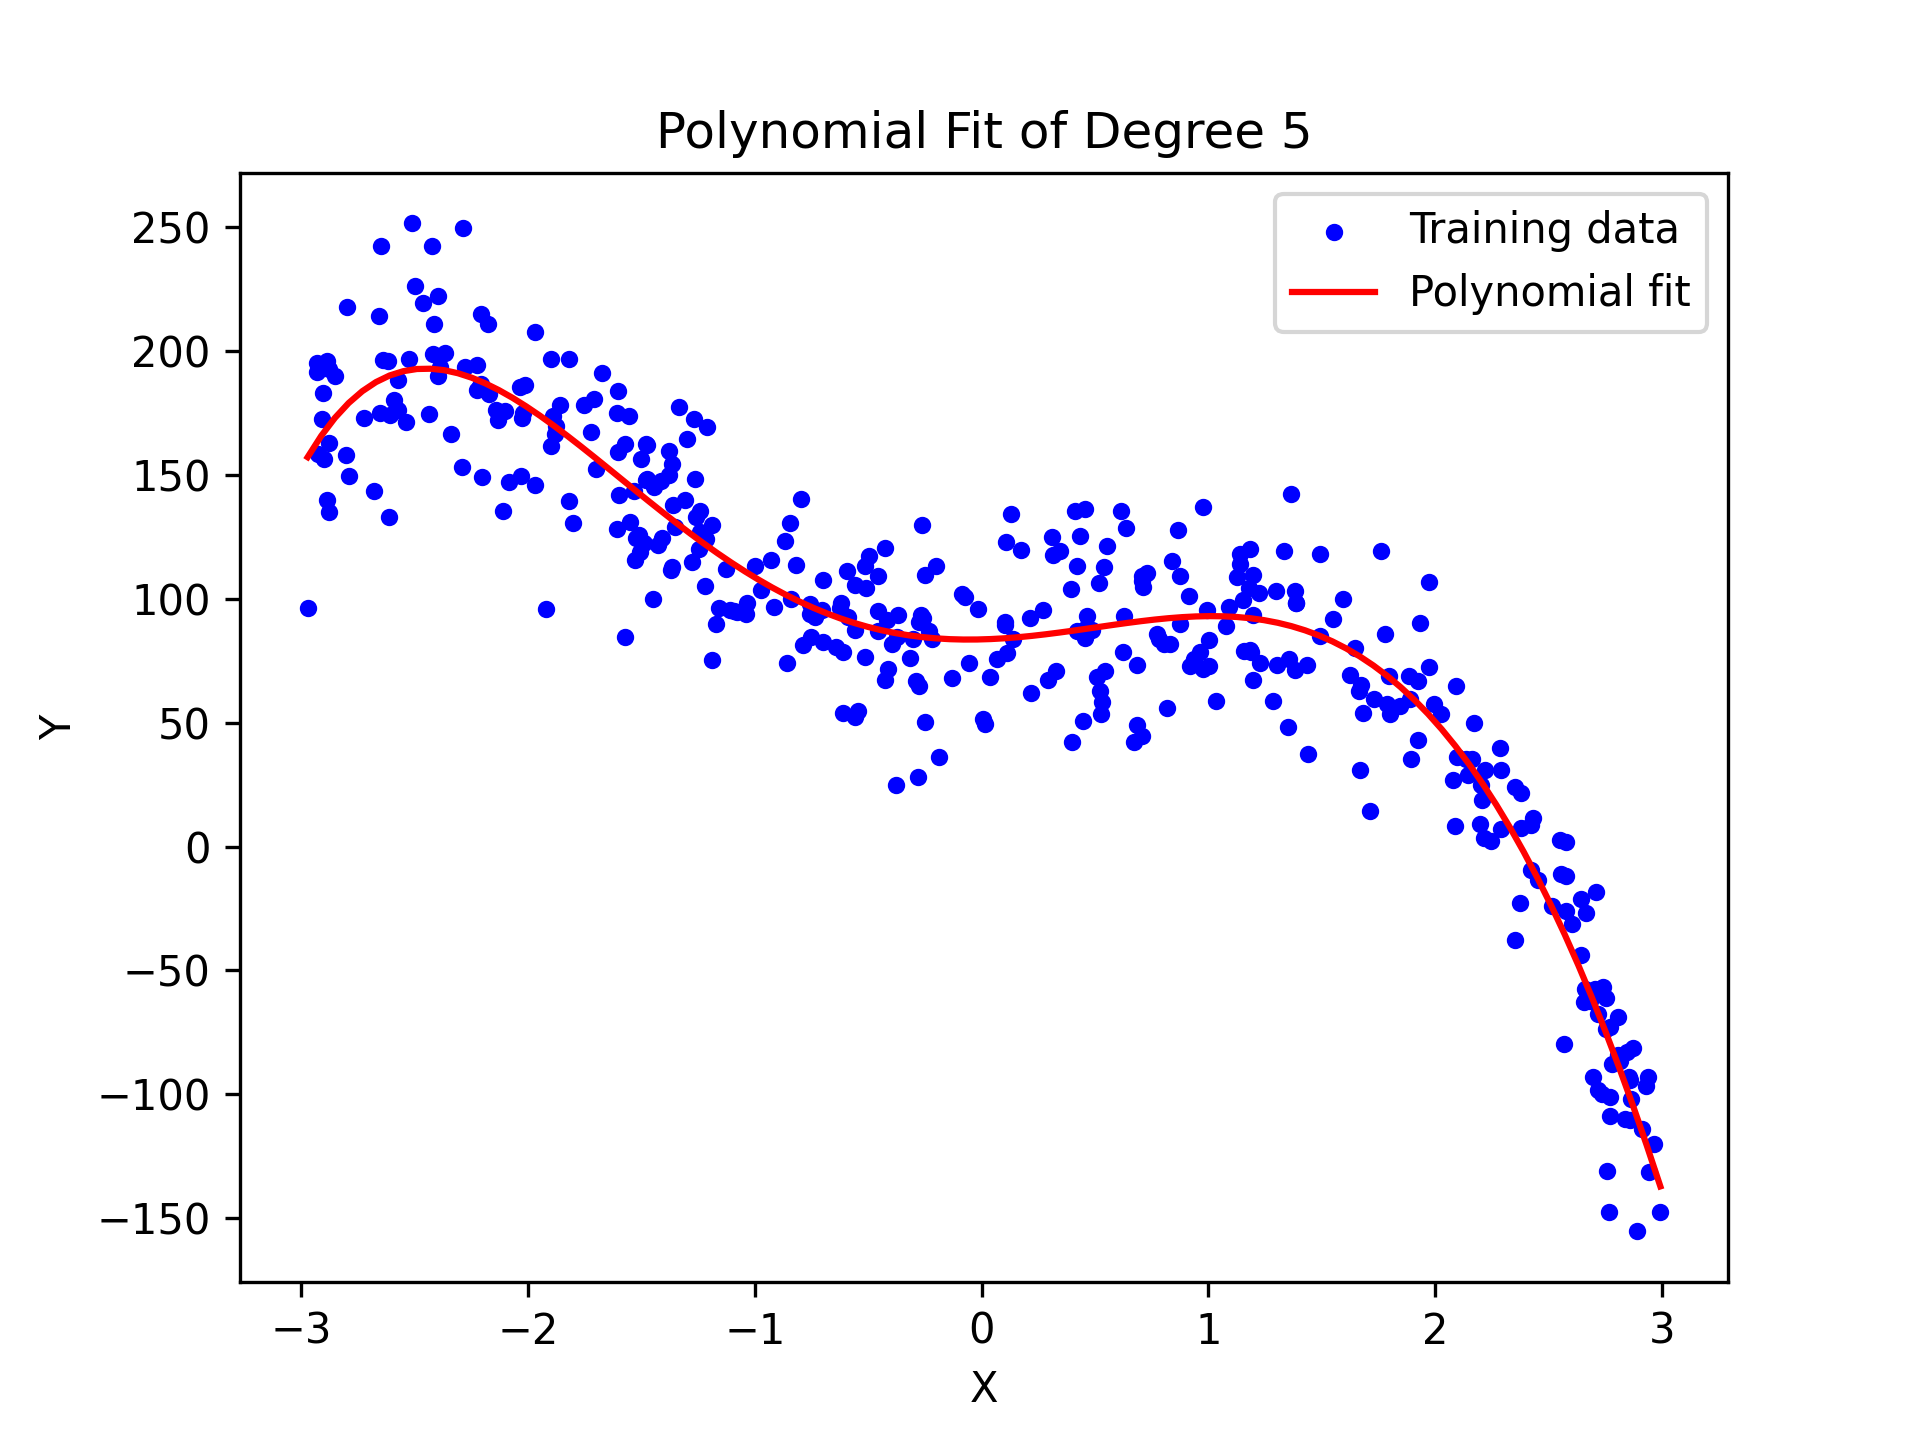
\includegraphics[width=0.5\textwidth]{./images/3/3_correctfit.png}
    \vspace{-10pt}
    \caption{Correct Fit}
\end{figure}
\vspace{-15pt}
\begin{figure}[H]
    \centering
    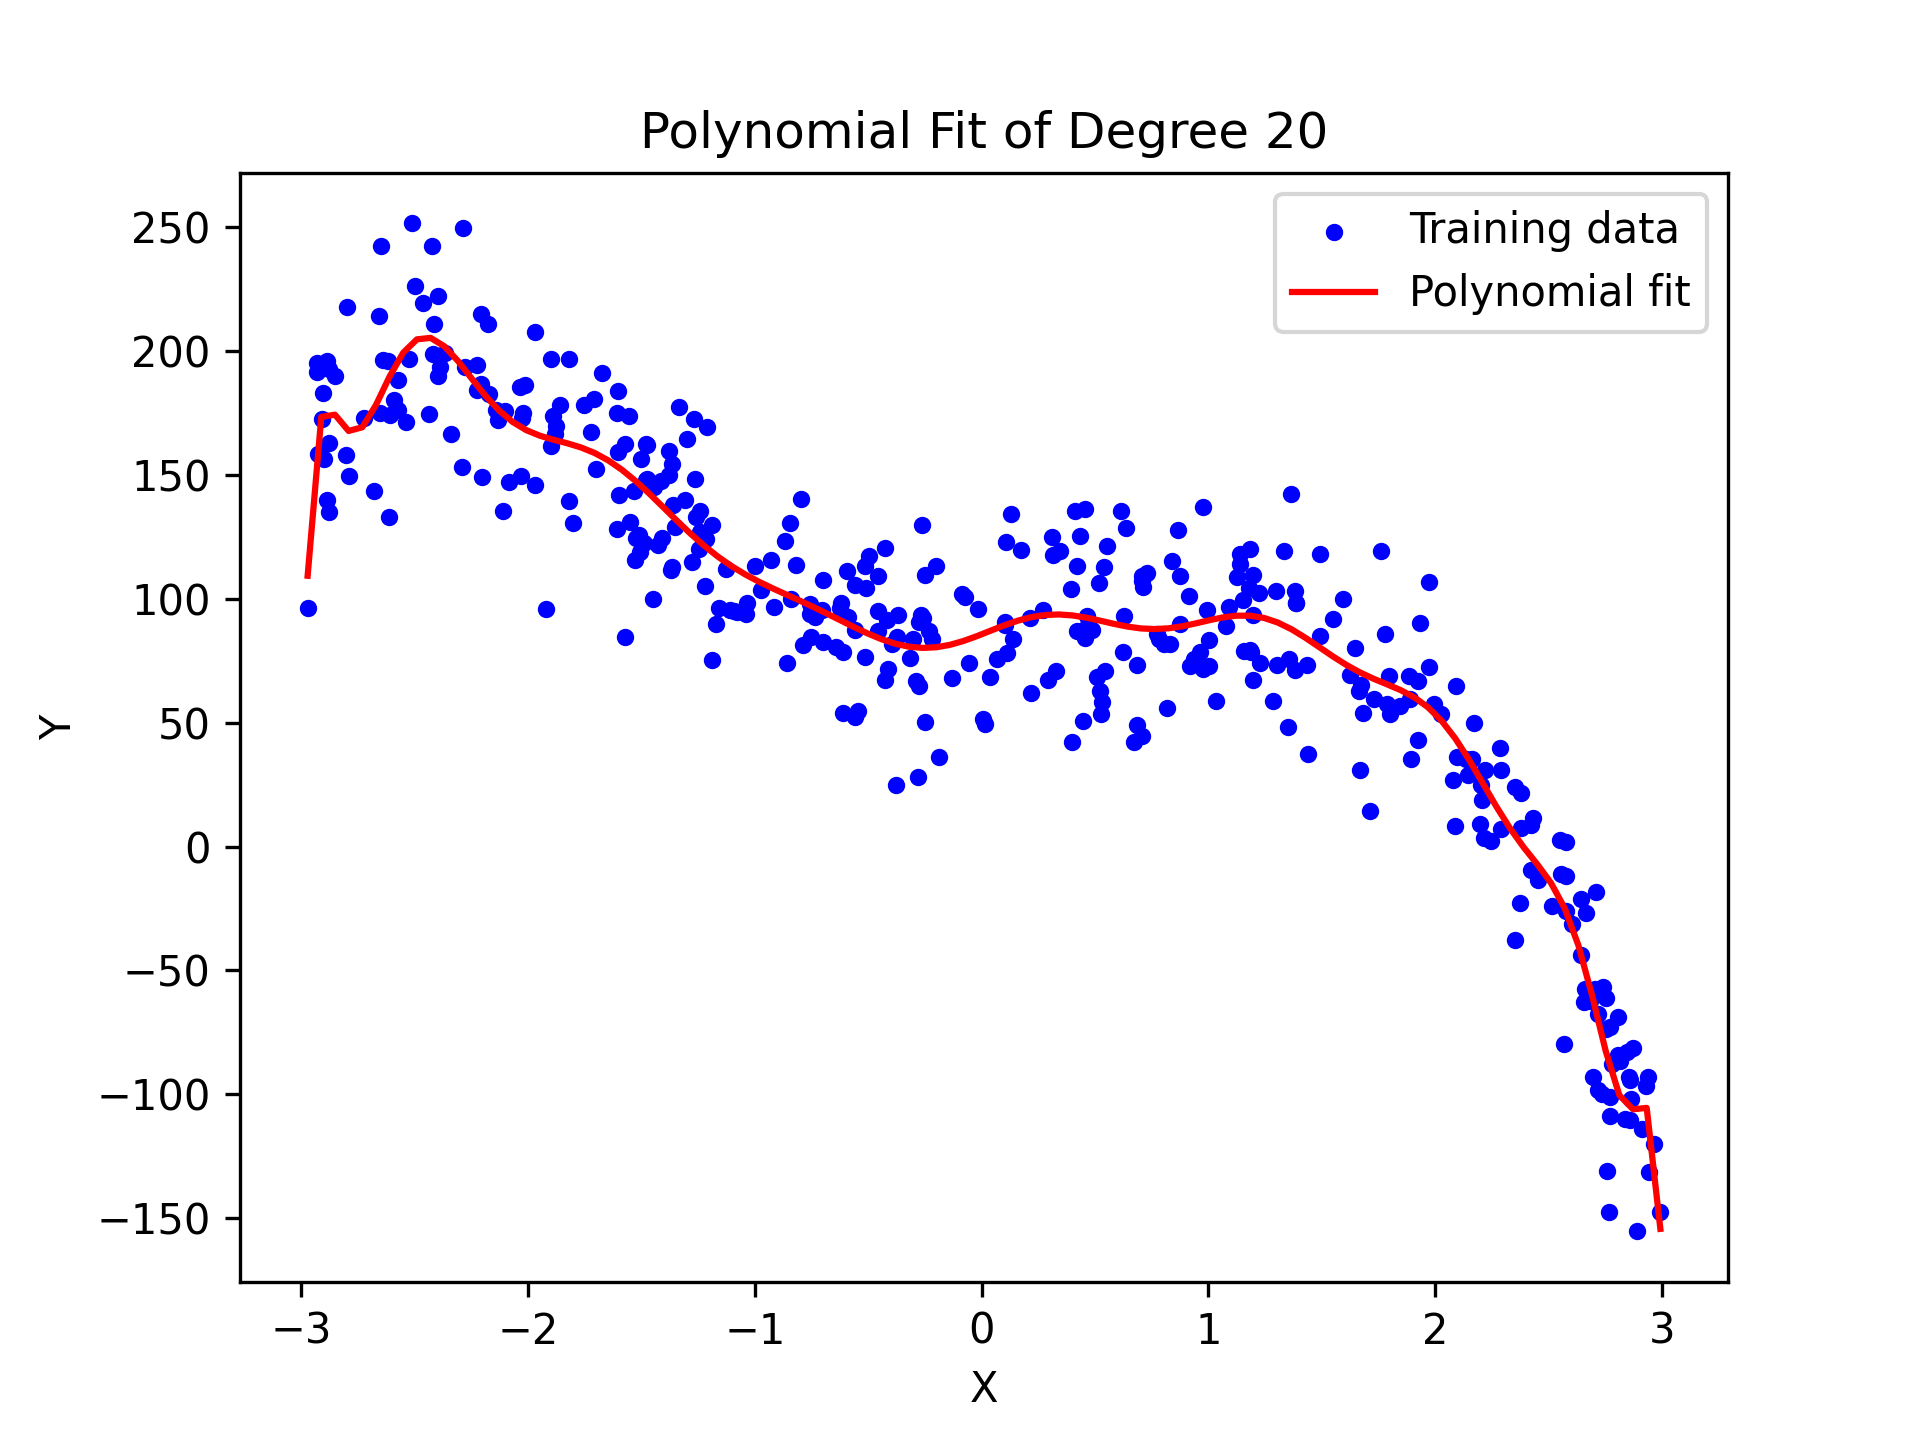
\includegraphics[width=0.5\textwidth]{./images/3/3_overfit.png}
     \vspace{-10pt}
    \caption{Overfit}
\end{figure}


\begin{center}    
    \begin{tabular}{|c|c|c|}
        \hline
        \bf{Degree Of Polynomial} & \bf{Type of Fit} & \bf{Coefficient Of Determination}\\
        \hline
        2 & Underfit & 0.8764 \\
        5 & Correct Fit & 0.9517\\
        20 & Overfit & 0.9545\\
        \hline
    \end{tabular} 
\end{center}